\chapter{Estimación de posición y velocidad}
	\section{Cálculo de la posición del objeto de interés}
Tal como se observa en la simulación de Gazebo (Figura 3.1), se decidió usar un sistema ortogonal derecho en la base de los pies como sistema de referencia que gobernará a todo el modelo.

\begin{figure}
	\centering		
	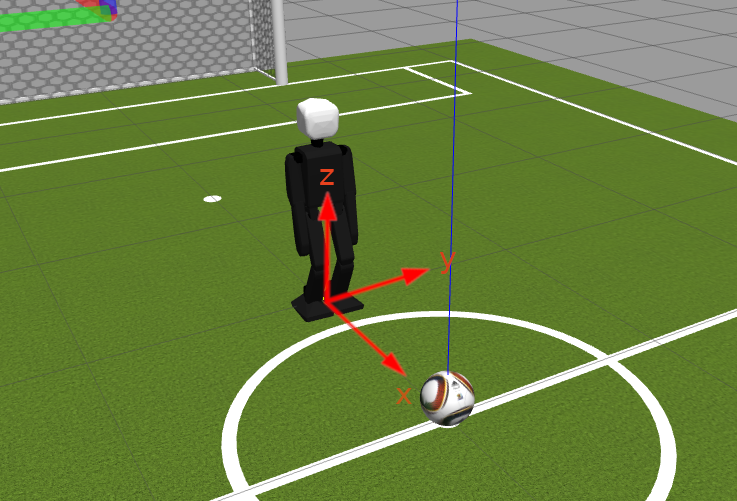
\includegraphics[scale=2]{images/robot_ejes.png}
	\caption{Representación del sistema de referencia usado en el robot.}		
\end{figure}

La cámara está localizada en la cabeza del humanoide, por lo que su centro
de visión se puede representar por un eje que va de la cámara al centroide del 
objeto, en este caso un balón de fútbol.
Para estimar la posición de un objeto que cruce por el centro de visión de la
cámara se necesita establecer un vector unitario:
\[\hat{u} = (u_x, u_y, u_z)\]
conocido en computación gráfica como vector \textit{look at}, (ver figura \ref{fig:LookAt}). Para obtener la ecuación vectorial de la recta paralela al vector \textit{look at} se toma un punto que contenga la recta, en este caso la posición de la cabeza en donde se encuentra la cámara: 

\begin{figure}
	\centering		
	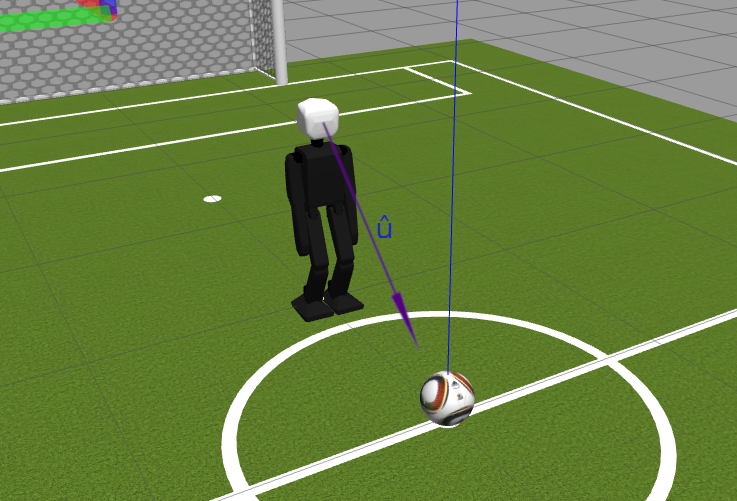
\includegraphics[scale=2]{images/robot_lookat.png}
	\caption{Representación del vector \textit{look at} utilizado en visión computacional.}		
	\label{fig:LookAt}
\end{figure}

\begin{equation}
\label{eq:LookAt}
r(\lambda) = (r_x, r_y, r_z)\quad +\quad \lambda (u_x, u_y, u_z)
\end{equation}


En donde $(r_x, r_y, r_z)$ es la posición en el espacio de la cámara utilizada, referida al sistema de referencia anteriormente mencionado. Se considera que el objetivo siempre estará en el suelo, por lo que el punto de intersección de la ecuación de la recta con el suelo hacen que la variable de altura sea igual a cero, conforme a la siguiente expresión:
\[r = (x, y, 0) = (r_x, r_y, r_z) + \lambda (u_x, u_y, u_z)\]
Despejando $\lambda$ del tercer término de la expresión anterior se obtiene:
\[\lambda = -\frac{r_z}{u_z}\]

De esta manera, substituyendo $\lambda$ en (\ref{eq:LookAt}), se obtiene:
\[x = r_x-\frac{r_z u_x}{u_z}\]
\[y = r_y-\frac{r_z u_y}{u_z}\]

Ya teniendo estas expresiones se procede a sustituir al vector unitario \textit{look at} con coordenadas esféricas, tal y como se observa en la siguiente expresión:
\begin{equation}
\label{eq:LookAtUnitary}
\hat{u}=(u_x, u_y, u_z)=(\sin{ \theta}\cos{\varphi},\sin{\theta}\sin{ \varphi},\cos{\theta})
\end{equation}

Sustituyendo la expresión (\ref{eq:LookAtUnitary}) dentro de los valores $x$ y $y$ da como resultado:
\[x=r_x - \frac{r_z \sin{ \theta} \cos{\varphi}}{\cos{\theta}}\]
\[y=r_y - \frac{r_z \sin{\theta} \sin{ \varphi}}{\cos{\theta}}\]

Utilizando la identidad trigonométrica:
\[\tan{\theta} = \frac{\sin{\theta}}{\cos{\theta}}\]

Las ecuaciones para obtener la posición del objetivo siempre y cuando $z=0$ son:
\begin{equation}
\label{eq:xBidimentionalPosition}
x=r_x - r_z \tan{\theta}  \cos{\varphi}
\end{equation}

\begin{equation}
\label{eq:yBidimentionalPosition}
y=r_y - r_z \tan{\theta} \sin{\varphi}
\end{equation}

No obstante, el objeto a considerar no es un objeto bidimensional, es un balón con forma esférica que está sobre el plano del suelo, debido a esto se pueden complementar las ecuaciones \ref{eq:xBidimentionalPosition} y \ref{eq:yBidimentionalPosition}, para obtener la posición (x,y,z) del centro del balón.

En la figura \ref{fig:ballProjection}(a) se observa un diagrama del balón en donde el vector \textit{look at} atravieza su centro e intersecta con el suelo en un punto en donde el balón no está. Esto representa un problema, ya que la posición en $x$ sufre una proyección, la cual incrementa mientras el balón tenga mayor radio. A esta proyección se le pondrá la variable $x_c$. Véase la figura \ref{fig:ballProjection}(b)


\begin{figure}
	\centering
	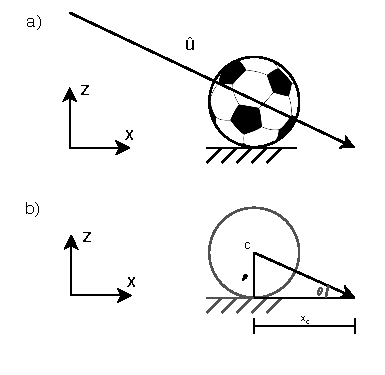
\includegraphics[scale=1.4]{images/ball_projection.pdf}
	\caption{(a) Bosquejo del vector \textit{look at} atravezando el centro del balón esférico; (b) Diagrama de la obtención de la distancia de proyección $x_c$.}
	\label{fig:ballProjection}
\end{figure}

Para obtener la magnitud de $x_c$ es necesario analizar el diagrama de la figura \ref{fig:ballProjection}(b), en donde $\theta$ es el ángulo \textit{pitch} y $\rho$ es el radio del balón. Así se puede obtener la siguiente igualdad:
\[\cot{\theta} = \frac{x_c}{\rho}\]\\

Despejando $x_c$
\[x_c = \rho \cot{\theta}\]

Debido a que $x_c$ se ve afectada también por la posición \textit{yaw} se deducen las siguientes igualdades para corregir el valor de la posición de $x$ y $y$ respectivamente:

\begin{equation}
\label{eq:xcForX}
x_{cx} = \rho \cot{\theta} \cos{\varphi}
\end{equation}

\begin{equation}
\label{eq:xcForY}
x_{cy} = \rho \cot{\theta} \sin{\varphi}
\end{equation}\\

De esta manera, se resta \ref{eq:xcForX}  a \ref{eq:xBidimentionalPosition} y \ref{eq:xcForY} a \ref{eq:yBidimentionalPosition}. Finalmente las ecuaciones resultantes son:

\[x = r_x - r_z \tan{\theta} \cos{\varphi} - \rho \cot{\theta} \cos{\varphi}\]
\[y = r_y - r_z \tan{\theta} \sin{\varphi} - \rho \cot{\theta} \sin{\varphi}\]
\[z = \rho \]


		
	\section{Estimación de estados mediante el Filtro de Kalman}
	Para poder impementar el Filtro de Kalman, se necesita primero tener un modelo matemático del sistema que se pretende tomar mediciones. Analizando el digrama de cuerpo libre de la Figura \ref{fig:dynamic_model} se puede hacer un análisis dinámico del balón utilizando la segunda ley de Newton.

\begin{equation}
\sum F = m \ddot{x}
\label{eq:second_law}
\end{equation}

\begin{equation}
F-f_{fricción} = m \ddot{x}
\label{eq:equivalency_1}
\end{equation}

Cambiando el nombre de las variables a corde de nuestro diagrama y tomando en como fuerza de fricción dinámica $f_{fricción} = \mu_d m g $ la igualdad de fuerzas es:
\begin{equation}
F- \mu_d m g = m  \frac{\mathrm{d} \dot{x}}{\mathrm{d} t}
\label{eq:equivalency_2}
\end{equation}
	
Donde $\mu_d$ es el coeficiente de fricción dinámica, $m$ es la masa del balón y $g$ es la aceleración de la gravedad. Debido a que la fuerza de fricción es la única que actúa sobre el balón, $F$ se iguala a cero, dejando el modelo el modelo cinemático de la expresión \ref{eq:mathematical_model_1}.

\begin{equation}
\frac{\mathrm{d} \dot{x}}{\mathrm{d} t} = - \mu_d g
\label{eq:mathematical_model_1}
\end{equation}

Despejando la variable $\dot{x}$ para se puede integrar la ecuación para obtener la velocidad en el tiempo $t$ del balón.
\begin{equation}
\int_{\dot{x}_0}^{\dot{x}} \mathrm{d} \dot{x} = -\mu_d g \int_{0}^{t} \mathrm{dt}  
\label{eq:mathematical_model_2}
\end{equation}

Resolviendo la ecuacion \ref{eq:mathematical_model_2} y despejando $\dot{x}$ se puede obtener la siguiente expresión:
\begin{equation}
\dot{x} = \dot{x}_{0} - \mu_d g t 
\label{eq:velocity_prediction}
\end{equation}

Una vez teniendo el modelo para predecir la velocidad del estado siguiente, se procede a integrar nuevamente para obtener su posición:
\begin{equation}
\int_{x_{0}}^{x} \mathrm{dx} = \int_{0}^{t} (\dot{x}_{0} - \mu_d g t) \mathrm{dt}
\label{eq:mathematical_model_4}
\end{equation}

Integrando y despejando $x$ se obtiene:
\begin{equation}
x = x_0 + \dot{x}_0 t - \frac{1}{2} \mu_d g t^2
\label{eq:position_prediction}
\end{equation}

%ESta ecuación es la solución de la ecuación diferencial que modela el movimiento
%De la eacuación 4.9 se tiene que:
Ya obtenida la ecuación para obtener la posición, despejamos la aceleración del modelo \ref{eq:equivalency_2}:
\begin{equation}
\ddot{x} = -\frac{1}{m}\mu_d m g + \frac{1}{m}F
\end{equation}

Pero F = 0. Es decir, que simplemente el balón comienza con $v_{0}$ diferente de cero y se va deteniendo.
Planteando esto en variables de estado:
\[ [x_1,x_2] = [x, \dot{x}]\]

En donde:
%\begin{eqnarray*}
\begin{equation}
\dot{x}_1 = x_2
\label{eq:state_variable_1}
\end{equation}

y 

\begin{equation}
\dot{x}_2 = -\frac{1}{m}\mu_d m g + \frac{1}{m}F
\label{eq:state_variable_2}
\end{equation}

%\end{eqnarray*}

\begin{figure}
\centering
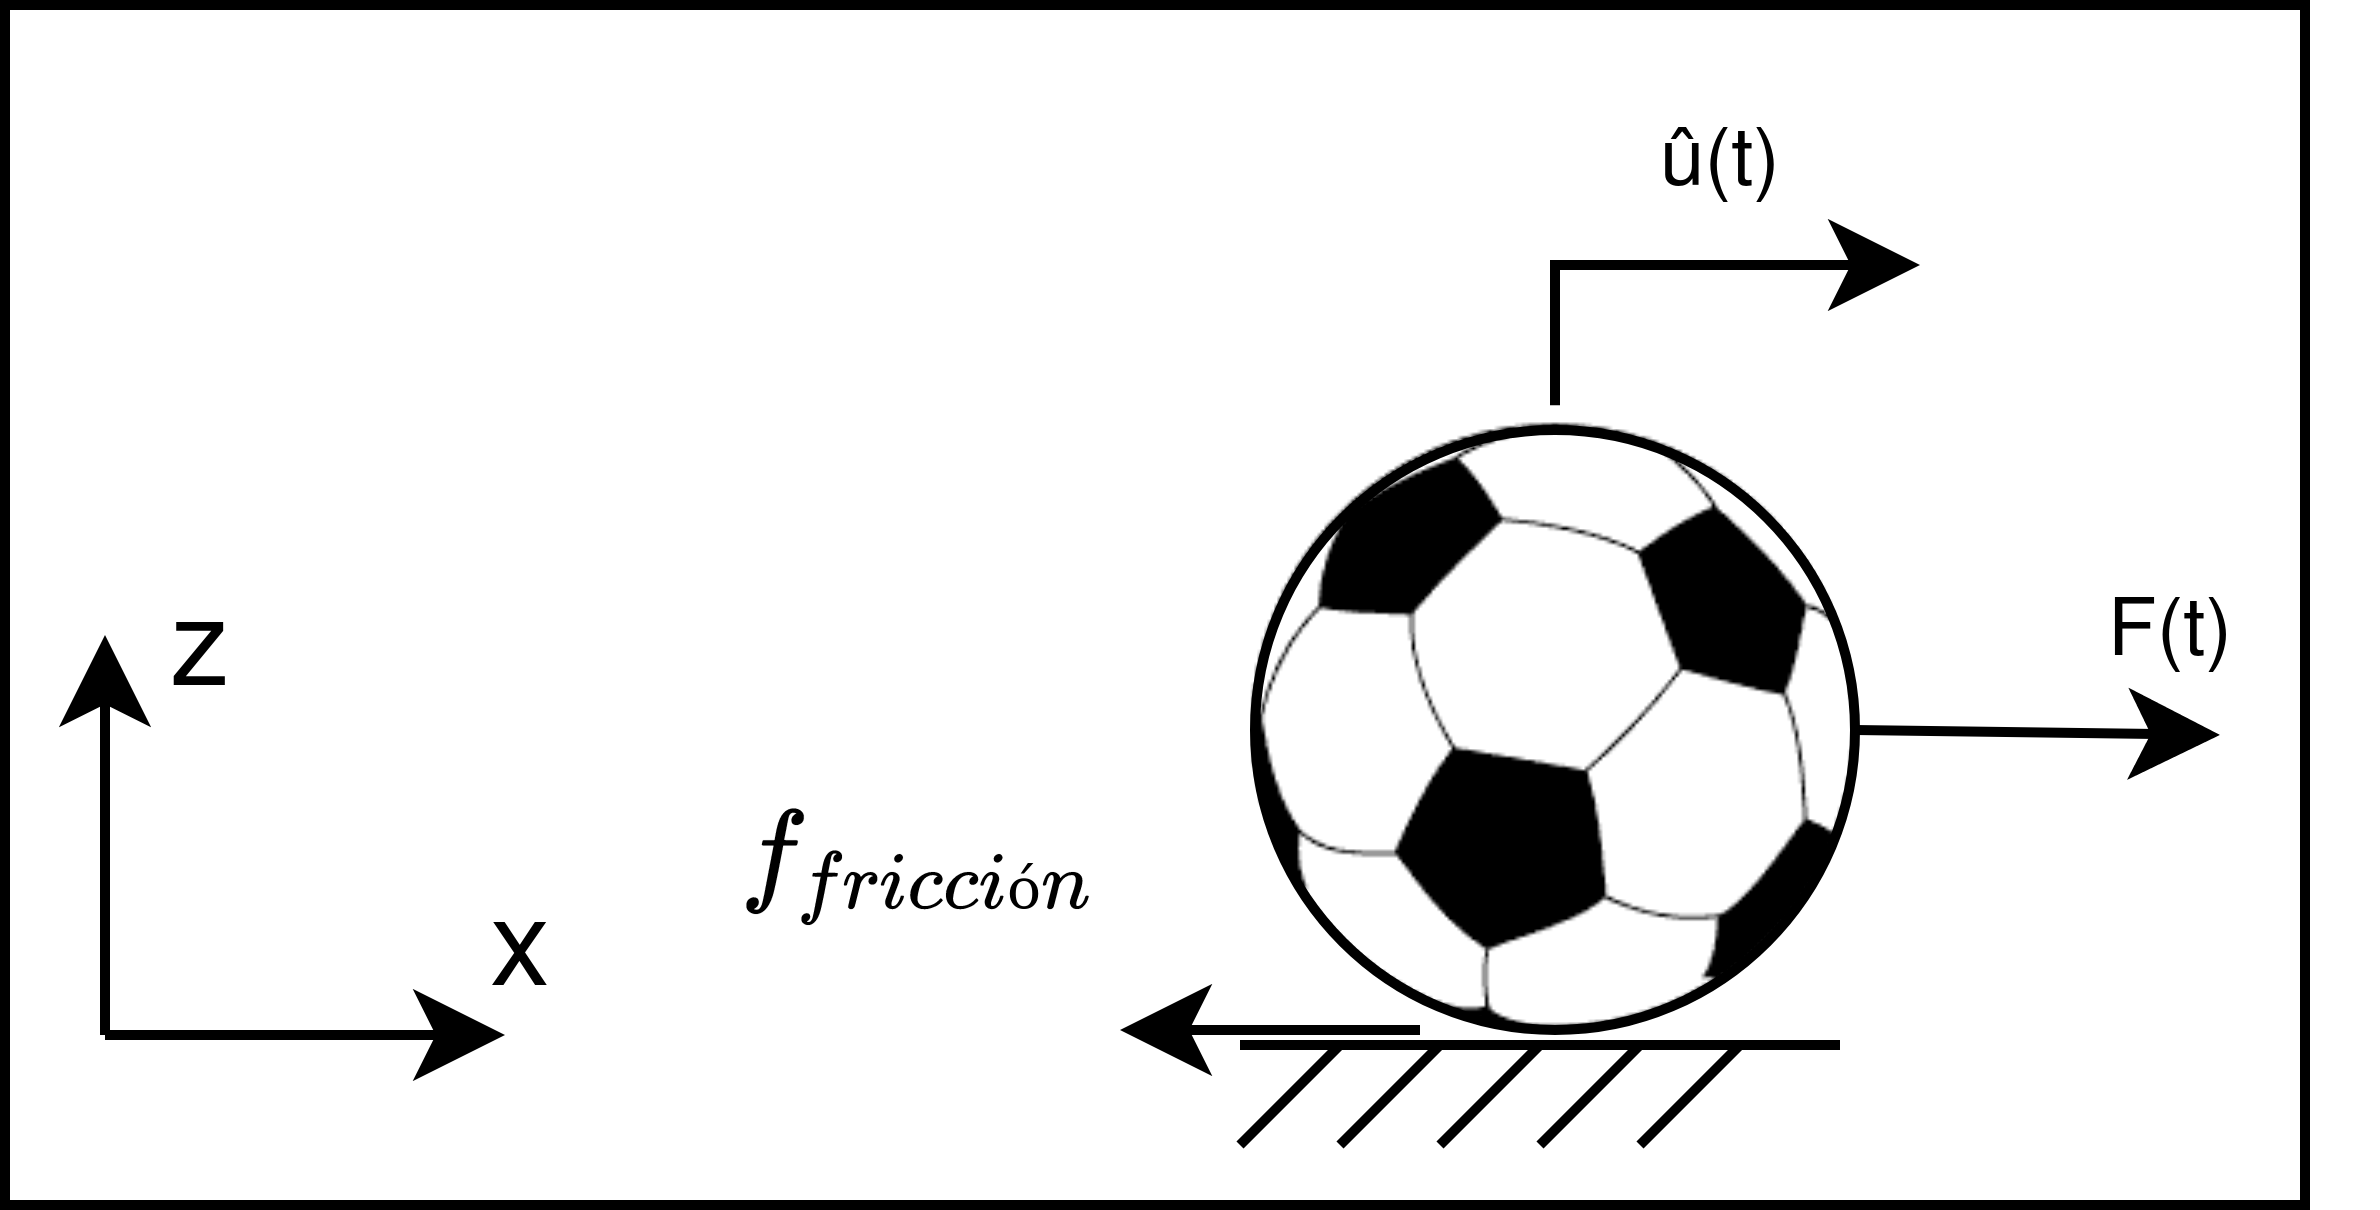
\includegraphics[scale=0.1]{images/dynamic_model.png}
\caption{Diagrama de cuerpo libre del objeto de interés}
\label{fig:dynamic_model}
\end{figure}

		\subsubsection*{Descripción del proceso de filtrado en el sistema}
Con el modelo dinámico que describe el movimiento del balón, se procede a escribir las ecuaciones matriciales del Filtro de Kalman (Véase la sección 2.4). De este modo, este filtro es una serie de pasos que iterativamente se deben ir completando para estimar posiciones y velocidades de un objeto en movimiento (Figura: \ref{fig:kalman_extended_diagram}).

\begin{figure}
\centering
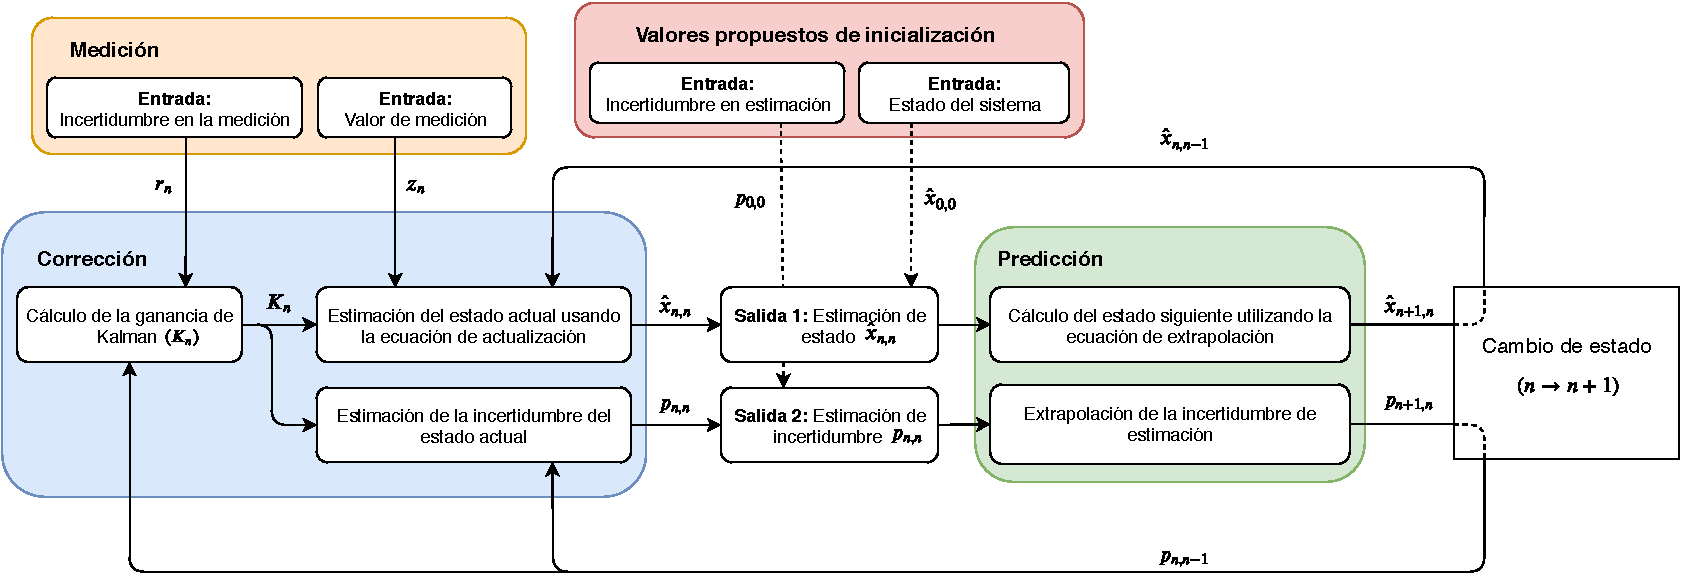
\includegraphics[scale=0.55]{images/kalman_extended_diagram.pdf}
\caption{Diagrama extendidio del funcionamiento paso a paso del Filtro de Kalman}
\label{fig:kalman_extended_diagram}
\end{figure}

		\subsubsection*{Modelado del sistema}
Para desarrollar las ecuaciones de extrapolación de estado se considerará que el balón se desplazará en el suelo sin elevarse o tener rebotes, por lo que el vector de estado $\hat{x}_n$ que describe la estimación de posición y velocidad en el plano \textit{(x, y)} es \ref{eq:state_vector}, siguiendo la nomenclatura que se vio en la sección 2.4.

\begin{equation}
\hat{x}_{n,n} = \begin{bmatrix}
x_{1_{n,n}}\\ 
y_{1_{n,n}}\\ 
x_{2_{n,n}}\\ 
y_{2_{n,n}}
\end{bmatrix}
\label{eq:state_vector}
\end{equation}

Dado que la única fuerza de entrada en el balón es la fricción, la cual depende del coeficiente de fricción dinámica y la gravedad el vector \textit{û} es representado como:
\begin{equation}
\hat{u}_n = \begin{bmatrix}
F_x\\
F_y
\end{bmatrix} = 
\begin{bmatrix}
0\\
0
\end{bmatrix}
\label{eq:input_signal}
\end{equation}


Como se vio en la sección 2.4, Figura \ref{fig:Kalman_scheme}, la ecuación de extrapolación de estado es:
\begin{equation}
\hat{x}_{n+1,n} = F \hat{x}_{n,n} + G \hat{u}_{n,n} + \omega_n
\label{eq:extrapolation_equation}
\end{equation}

No obstante, con la deducción de la ecuación de posición, el modelo no es lineal, por lo que la ecuación \ref{eq:extrapolation_equation}, usando el Filtro de Kalman Extendido se transforma en:

\begin{equation}
\hat{x}_{n+1,n} = f(\hat{x}_{n,n}, \hat{u}_{n,n}) + \omega_n
\label{eq:efk}
\end{equation}


\ref{eq:state_variable_2} es el modelo en variables de estado, continuo. Para el EKF se discretiza este modelo. Y la señal de entrada F = 0. 

El modelo discreto del sistema con ruido es:
\begin{eqnarray*}
x_{1_{n+1,n}} &=& x_{1_{n,n}} + \Delta t x_{2_{n,n}} + \omega_1\\ %Modelo1
y_{1_{n+1,n}} &=& y_{1_{n,n}} + \Delta t y_{2_{n,n}} + \omega_2\\ %Modelo2
x_{2_{n+1,n}} &=& x_{2_{n,n}} - \Delta t \frac{1}{m}\mu_d m g + \frac{1}{m} F_x + \omega_3\\ %Modelo3
y_{2_{n+1,n}} &=& y_{2_{n,n}} - \Delta t \frac{1}{m}\mu_d m g + \frac{1}{m} F_y + \omega_4 %Modelo4
\end{eqnarray*}

O escrito en su forma matricial:

\begin{equation}
\hat{x}_{n+1,n} =
\begin{bmatrix}
1 & 0 & \Delta t & 0\\ 
0 & 1 & 0 & \Delta t\\
0 & 0 & 1 & 0\\
0 & 0 & 0 & 1\\
\end{bmatrix}
\begin{bmatrix}
x_{1_{n,n}}\\ 
y_{1_{n,n}}\\
x_{2_{n,n}}\\
y_{2_{n,n}}
\end{bmatrix}
+
\begin{bmatrix}
0 \\
0 \\
- \Delta t \mu_d g \\
- \Delta t \mu_d g 
\end{bmatrix}
+
\begin{bmatrix}
\omega_1 \\ 
\omega_2 \\
\omega_3 \\
\omega_4
\end{bmatrix}
\end{equation}	

$\Omega = [\omega_1, ... ,\omega_4]$ es un vector de ruido con distribución normal, media cero, y matriz de covarianza $Q\in \mathbb{R}^{4\times 4}$.

Para estas ecuaciones se tienen dos entradas, que son las posiciones en $x$ y $y$ con su respectiva insertidumbre de medición.

\begin{eqnarray*}
z_1 &=& x_1 + v_1\\
z_2 &=& y_1 + v_2
\end{eqnarray*}

o en forma matricial:
\begin{equation}
\hat{z} =
\begin{bmatrix}
x_1 \\ 
y_1
\end{bmatrix}
+
\begin{bmatrix}
v_1 \\ 
v_2
\end{bmatrix}
\end{equation}

$V = [v_1, v_2]$ es el vector de ruido de la medición, considerando que tiene una distribución normal, media cero y matriz de covarianza $R\in \mathbb{R}^{2\times 2}$.

Se definirá como matriz de predicción F a la matriz:

\begin{equation}
F =
\begin{bmatrix}
1 & 0 & \Delta t & 0\\ 
0 & 1 & 0 & \Delta t\\
0 & 0 & 1 & 0\\
0 & 0 & 0 & 1\\
\end{bmatrix}
\end{equation}

		\subsubsection*{Extrapolación de la incertidumbre de estimación}
	El proceso de estimación en el Filtro de Kalman es un modelo basado en la \textit{esperanza} de una serie de variables aleatorias para obtener el valor \textit{oculto} que se considera el real. Este proceso de filtrado considera que todos los errores tanto en medición como en estimación tienen una \textit{distribución gaussiana} por lo que cada incertidumbre tiene que expresarse como la varianza de una recompilación de datos. De una manera análoga a la predicción de posición y velocidad en un tiempo $\Delta t$ la incertidumbre de estimación se puede calcular con la siguiente ecuación matricial:
	
\begin{equation}
P_{n+1,n} = F P_{n,n} F^T + Q
\label{eq:extrapolation_process_cov_matrix}
\end{equation}

Donde P es una matriz diagonal definida como: 
\begin{equation}
\hat{P}_{n,n} =
\begin{bmatrix}
Px_{1_{n,n}} & 0 & 0 & 0\\ 
0 & Py_{1_{n,n}} & 0 & 0\\ 
0 & 0 & Px_{2_{n,n}} & 0\\ 
0 & 0 & 0 & Py_{2_{n,n}}
\end{bmatrix}
\end{equation}	

Q es una matriz diagonal cuadrada: 
\begin{equation}
Q =
\begin{bmatrix}
q_{x_1} & 0 & 0 & 0\\ 
0 & q_{y_1} & 0 & 0\\ 
0 & 0 & q_{x_2} & 0\\ 
0 & 0 & 0   & q_{y_2}
\end{bmatrix}
\end{equation}	

Resolviendo la ecuación \ref{eq:extrapolation_process_cov_matrix}, tomando sólamente los valores de la diagonal principal, dan como resultados individuales las siguientes ecuaciones:
	
\begin{eqnarray*}
	Px_{1_{n+1,n}} = Px_{1_{n,n}} + \Delta t^{2} Px_{2_{n,n}} + q_{x_1}\\
	Py_{1_{n+1,n}} = Py_{1_{n,n}} + \Delta t^{2} Py_{2_{n,n}} + q_{y_1}\\
	Px_{2_{n+1,n}} = Px_{2_{n,n}} 				    		  + q_{x_2}\\
	Py_{2_{n+1,n}} = Py_{2_{n,n}}							  + q_{y_2}\\
\end{eqnarray*}

		\subsubsection*{Obtención de la ganancia de Kalman}
	Una vez teniendo la predicción del estado siguiente, es posible comparar las mediciones con las predicciones préviamente hechas para hacer un proceso de corrección. Para esto es necesario obtener el peso de la ganancia de Kalman que se describe con la siguiente ecuación:
\begin{equation}
	K_n = P_{n,n-1} H^T (H P_{n,n-1} H^T +V R_n V^T)^{-1}
	\label{eq:kalman_gain}
\end{equation}

Por las dimensiones de la matriz $P$ y por el hecho que la entrada $z$ sólo tiene dos valores, la matriz de observación $H$ tiene que ser una matriz de cuatro por cuatro con los siguientes valores:

\begin{equation}
	H =
	\begin{bmatrix}
	1 & 0 & 0 & 0\\
	0 & 1 & 0 & 0\\
	0 & 0 & 0 & 0\\
	0 & 0 & 0 & 0
	\end{bmatrix}
\end{equation}

Como ya se había mencionado, $R_n$ es una matriz cuadrada de $2x2$ la cual contiene la covarianza del ruido:
\begin{equation}
	R_n = 
	\begin{bmatrix}
	R_x & 0\\
	0  & R_y
	\end{bmatrix}
\end{equation} 
y la matriz $V$ sirve para que la matriz de covarianza de la medición se redimensione haciendo posible las operaciones de la ecuación \ref{eq:kalman_gain}:
\begin{equation}
	V=
	\begin{bmatrix}
	1 & 0\\
	0 & 1\\
	0 & 0\\
	0 & 0
	\end{bmatrix}
\end{equation}

Por lo tanto, la operación \ref{eq:kalman_gain} da como resultado una matriz de $4x4$ que se observa de la siguiente manera:

\begin{equation}
	K = 
	\begin{bmatrix}
	k_1 & 0 & 0 & 0   \\
	 0  & k_2 & 0 & 0 \\
	 0  & 0   & 0 & 0 \\
	 0  & 0   & 0 & 0
	\end{bmatrix}
	=
	\begin{bmatrix}
	\frac{Px_{1_{n,n}}}{(Px_{1_{n,n}} + R_x)} & 0 & 0 & 0\\
	                                        0 & \frac{Py_{1_{n,n}}}{(Py_{1_{n,n}} + R_y)} & 0 & 0\\
	                                        0 & 0 & 0 & 0\\
											0 & 0 & 0 & 0
	\end{bmatrix}
\end{equation}

		\subsubsection*{Corrección de estimación de estado}
	Con cada nueva medición, se procede a hacer la corrección del estado presente, haciendo uso del la ganancia del filtro para poder \textit{decidir} si es más fiable la medición o la predicción.

\begin{equation}
\hat{x}_{n,n} = \hat{x}_{n,n-1} + K_n(z_n - H \hat{x}_{n,n-1})
\label{eq:prediction_eq}
\end{equation}

A primera instancia, se deduce que el vector de entrada $z_n$ es de dos elementos, no obstante, para lograr que se pueda sumar dentro de la ecuación \ref{eq:prediction_eq} se requiere que el vector tenga la siguiente forma:

\begin{equation}
	z_n =
	\begin{bmatrix}
		z_1\\
		z_2\\
		 0 \\
		 0
	\end{bmatrix}
\end{equation}
	
		\subsubsection*{Corrección del error de covarianza}
	De una manera muy similar el error de covarianza se puede actualizar utilizando la ganancia de Kalman:

\begin{equation}
P_{n,n} = (I - K_n H) P_{n,n-1}
\end{equation}

	\section{Obtencion de los parametros}
		\subsection*{Coeficiente de fricción dinámica}
	De acuerdo con la ecuación \ref{eq:position_prediction} y como se vio a lo largo de su deducción, el modelo de la posición del balón respecto al tiempo, depende únicamente del coeficiente de fricción dinámica entre el balón y el material el cual se desplaza. Para obtener dicho coeficiente se optó por la solución más simple, la cual consiste en medir diréctamente la fuerza que se opone al desplazamiento, por medio de un dinamómetro de resorte marca \textit{Pasco} con rango de 0 a 10[N] y una resolución de 0.1[N]. Véase la figura \ref{fig:dynamometer}. 
	
\begin{figure}
\centering
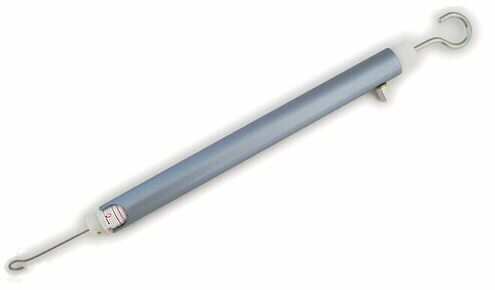
\includegraphics[scale=0.4]{images/dynamometer.jpg}
\caption{Dinamómetro de resorte utilizado para obtener la fuerza de fricción}
\label{fig:dynamometer}
\end{figure}	

	Las medidas del dinamómetro del peso del balón dio $2.2[N]$, de la fuerza de fricción estática $F_{e} = 1.5[N]$ y de la fuerza de fricción dinámica $F_{d} = 0.8[N]$. 

	Por lo que se puede aplicar la segunda ley de Newton (de manera simplificada) para despejar el coeficiente de fricción deseado:
\begin{equation}
F_d = N\mu_d 
\end{equation}
	En donde $N$ es la fuerza normal a la superficie con la misma magnitud del peso del balón (por considerar que se está desplazando de manera horizontal). Por tanto la fuerza de fricción dinámica es:
	
\begin{equation}
	\mu_d = \frac{F_d}{N}
	      = 0.3636		
\end{equation}
	
		\subsection*{Parámetros de Kalman}
		Como en muchos sistemas de control, siempre es mejor variar los parámetros conforme se hagan pruebas, a fin de obtener resultados más óptimos a lo que uno espera. Siendo así, los siguientes parámetros son los que se fueron variando con cada prueba y se decidió que fueron los mejores para filtrar los diversos errores inherentes al sistema. 
		

		\subsubsection*{Matriz de covarianza del ruido del proceso}
\begin{equation}
Q = \begin{bmatrix}
0.000001 & 0 & 0 & 0\\ 
0        & 0.000001 & 0        & 0\\ 
0        & 0        & 0.000001 & 0\\ 
0.0      & 0        & 0        & 0.000001
\end{bmatrix}
\label{eq:process_noise_matrix}
\end{equation}

		\subsubsection*{Matriz de error de medición}
\begin{equation}
R_n = \begin{bmatrix}
0.025 & 0\\ 
0     & 0.025
\end{bmatrix}
\label{eq:noise_measurement}
\end{equation}

		\subsubsection*{Valores iniciales de entrada}
		Debido a que el algoritmo se encarga de converger los valores de entrada con el valor esperado de cada estado, por lo tanto no son de mucha importancia los valores $\hat{x}_{0,0}$ y $\hat{P}_{0,0}$.
\begin{equation}
\hat{x}_{0,0} = \begin{bmatrix}
-0.3\\ 
-0.3\\ 
0.3\\ 
0.3
\end{bmatrix}
\label{eq:initial_state_vector}
\end{equation}

\begin{equation}
P_{0,0} 
=
\begin{bmatrix}
0.1 & 0   & 0   & 0\\ 
0   & 0.1 & 0   & 0\\
0   & 0   & 0.1 & 0\\
0   & 0   & 0   & 0.1
\end{bmatrix}
\label{eq:initial_cov_vector}
\end{equation}	